\documentclass[twoside]{book}

% Packages required by doxygen
\usepackage{fixltx2e}
\usepackage{calc}
\usepackage{doxygen}
\usepackage[export]{adjustbox} % also loads graphicx
\usepackage{graphicx}
\usepackage[utf8]{inputenc}
\usepackage{makeidx}
\usepackage{multicol}
\usepackage{multirow}
\PassOptionsToPackage{warn}{textcomp}
\usepackage{textcomp}
\usepackage[nointegrals]{wasysym}
\usepackage[table]{xcolor}

% NLS support packages
Portuguese
% Font selection
\usepackage[T1]{fontenc}
\usepackage[scaled=.90]{helvet}
\usepackage{courier}
\usepackage{amssymb}
\usepackage{sectsty}
\renewcommand{\familydefault}{\sfdefault}
\allsectionsfont{%
  \fontseries{bc}\selectfont%
  \color{darkgray}%
}
\renewcommand{\DoxyLabelFont}{%
  \fontseries{bc}\selectfont%
  \color{darkgray}%
}
\newcommand{\+}{\discretionary{\mbox{\scriptsize$\hookleftarrow$}}{}{}}

% Page & text layout
\usepackage{geometry}
\geometry{%
  a4paper,%
  top=2.5cm,%
  bottom=2.5cm,%
  left=2.5cm,%
  right=2.5cm%
}
\tolerance=750
\hfuzz=15pt
\hbadness=750
\setlength{\emergencystretch}{15pt}
\setlength{\parindent}{0cm}
\setlength{\parskip}{3ex plus 2ex minus 2ex}
\makeatletter
\renewcommand{\paragraph}{%
  \@startsection{paragraph}{4}{0ex}{-1.0ex}{1.0ex}{%
    \normalfont\normalsize\bfseries\SS@parafont%
  }%
}
\renewcommand{\subparagraph}{%
  \@startsection{subparagraph}{5}{0ex}{-1.0ex}{1.0ex}{%
    \normalfont\normalsize\bfseries\SS@subparafont%
  }%
}
\makeatother

% Headers & footers
\usepackage{fancyhdr}
\pagestyle{fancyplain}
\fancyhead[LE]{\fancyplain{}{\bfseries\thepage}}
\fancyhead[CE]{\fancyplain{}{}}
\fancyhead[RE]{\fancyplain{}{\bfseries\leftmark}}
\fancyhead[LO]{\fancyplain{}{\bfseries\rightmark}}
\fancyhead[CO]{\fancyplain{}{}}
\fancyhead[RO]{\fancyplain{}{\bfseries\thepage}}
\fancyfoot[LE]{\fancyplain{}{}}
\fancyfoot[CE]{\fancyplain{}{}}
\fancyfoot[RE]{\fancyplain{}{\bfseries\scriptsize Gerado por Doxygen }}
\fancyfoot[LO]{\fancyplain{}{\bfseries\scriptsize Gerado por Doxygen }}
\fancyfoot[CO]{\fancyplain{}{}}
\fancyfoot[RO]{\fancyplain{}{}}
\renewcommand{\footrulewidth}{0.4pt}
\renewcommand{\chaptermark}[1]{%
  \markboth{#1}{}%
}
\renewcommand{\sectionmark}[1]{%
  \markright{\thesection\ #1}%
}

% Indices & bibliography
\usepackage{natbib}
\usepackage[titles]{tocloft}
\setcounter{tocdepth}{3}
\setcounter{secnumdepth}{5}
\makeindex

% Hyperlinks (required, but should be loaded last)
\usepackage{ifpdf}
\ifpdf
  \usepackage[pdftex,pagebackref=true]{hyperref}
\else
  \usepackage[ps2pdf,pagebackref=true]{hyperref}
\fi
\hypersetup{%
  colorlinks=true,%
  linkcolor=blue,%
  citecolor=blue,%
  unicode%
}

% Custom commands
\newcommand{\clearemptydoublepage}{%
  \newpage{\pagestyle{empty}\cleardoublepage}%
}

\usepackage{caption}
\captionsetup{labelsep=space,justification=centering,font={bf},singlelinecheck=off,skip=4pt,position=top}

%===== C O N T E N T S =====

\begin{document}

% Titlepage & ToC
\hypersetup{pageanchor=false,
             bookmarksnumbered=true,
             pdfencoding=unicode
            }
\pagenumbering{roman}
\begin{titlepage}
\vspace*{7cm}
\begin{center}%
{\Large Frog\+Race }\\
\vspace*{1cm}
{\large Gerado por Doxygen 1.8.11}\\
\end{center}
\end{titlepage}
\clearemptydoublepage
\tableofcontents
\clearemptydoublepage
\pagenumbering{arabic}
\hypersetup{pageanchor=true}

%--- Begin generated contents ---
\chapter{Frog\+Race}
\label{md_README}
\hypertarget{md_README}{}
\begin{quote}
Frog\+Race \end{quote}


Este repositório contém\+:


\begin{DoxyEnumerate}
\item Informações sobre a configuração
\item Instruções de compilação
\item Instruções de execução
\item Informações sobre localização dos códigos que serão avaliados
\end{DoxyEnumerate}

\subsection*{Tabela de Conteúdos}


\begin{DoxyItemize}
\item \href{#configuração}{\tt Configuração}
\item \href{#compilação}{\tt Compilação}
\item \href{#execução}{\tt Execução}
\item \href{#códigos-avaliados}{\tt Códigos Avaliados}
\begin{DoxyItemize}
\item \href{#passos-1-2}{\tt Passos 1, 2}
\item \href{#passos-3-4-5}{\tt Passos 3, 4 e 5}
\item \href{#passo-6}{\tt Passo 6}
\end{DoxyItemize}
\end{DoxyItemize}

\subsection*{Configuração}

Para o desenvolvimento deste projeto foi utilizado apenas as bibliotecas padrão do c++, $<$iostream$>$, $<$string$>$, $<$random$>$, $<$fstream$>$, $<$istream$>$ e $<$ostream$>$. Com excessão da T\+AD Lista utilizada, que foi implementada anteriormente e depois incluída no projeto com seu respectivo Iterador.

\subsection*{Compilação}

Para compilar o programa é necessário que existam as demais pastas do projeto. Caso elas não existam, execute o comando \textquotesingle{}make dir\textquotesingle{} a partir da pasta raíz do projeto. Também é necessária a existência dos arquivos corridas.\+csv e sapos.\+csv dentro da pasta data. Finalmente, basta compilar o programa executando o comando \textquotesingle{}make\textquotesingle{} ou \textquotesingle{}make Frog\+Race\textquotesingle{}.

\subsection*{Execução}

O programa ficará localizado na pasta bin. Para executá-\/lo a partir da pasta raíz do projeto, execute o comando \textquotesingle{}./bin/\+Frog\+Race\textquotesingle{}.

\subsection*{Códigos Avaliados}

Os passos 1, 2 e 6 estão localizados no arquivo \hyperlink{dataManager_8h}{data\+Manager.\+h}. Os passos 3, 4, 5 estão localizados ni arquivo \hyperlink{main_8cpp}{main.\+cpp}.

\subsection*{Passos 1, 2}

Linhas 76-\/79. Função que funciona para ambas classes \hyperlink{classSapo}{Sapo} e \hyperlink{classCorrida}{Corrida}.

\subsection*{Passos 3, 4 e 5}

Passo 3\+: Linhas 184-\/192 Descrevem a função que exibe o menu na tela. Linhas 204-\/233 Contém o loop lógico do menu principal. Passo 4\+: Linhas 152-\/168 Descrevem a função que retorna a escolha da corrida. Passo 5\+: Linhas 95-\/135 Descrevem a função que determina a lógica da corrida propriamente dita.

\subsection*{Passo 6}

Criar o \hyperlink{classSapo}{Sapo}\+: Linhas 128-\/137. Criar a \hyperlink{classCorrida}{Corrida}\+: Linhas 146-\/163. Salvar \hyperlink{classSapo}{Sapo}\+: Linhas 108-\/119. 
\chapter{Índice dos componentes}
\section{Lista de componentes}
Lista de classes, estruturas, uniões e interfaces com uma breve descrição\+:\begin{DoxyCompactList}
\item\contentsline{section}{\hyperlink{classCorrida}{Corrida} }{\pageref{classCorrida}}{}
\item\contentsline{section}{\hyperlink{classIterator}{Iterator$<$ T, Y $>$} }{\pageref{classIterator}}{}
\item\contentsline{section}{\hyperlink{classList}{List$<$ T $>$} }{\pageref{classList}}{}
\item\contentsline{section}{\hyperlink{classNode}{Node$<$ T $>$} }{\pageref{classNode}}{}
\item\contentsline{section}{\hyperlink{classSapo}{Sapo} \\*Classe que representa um \hyperlink{classSapo}{Sapo} }{\pageref{classSapo}}{}
\end{DoxyCompactList}

\chapter{Índice dos ficheiros}
\section{Lista de ficheiros}
Lista de todos os ficheiros documentados com uma breve descrição\+:\begin{DoxyCompactList}
\item\contentsline{section}{include/{\bfseries corrida.\+h} }{\pageref{corrida_8h}}{}
\item\contentsline{section}{include/\hyperlink{dataManager_8h}{data\+Manager.\+h} \\*Responsável por carregar e salvar as informaçoes das classes em arquivo }{\pageref{dataManager_8h}}{}
\item\contentsline{section}{include/\hyperlink{fileHandler_8h}{file\+Handler.\+h} \\*Responsável por manipular os arquivos C\+SV }{\pageref{fileHandler_8h}}{}
\item\contentsline{section}{include/{\bfseries lista.\+h} }{\pageref{lista_8h}}{}
\item\contentsline{section}{include/\hyperlink{sapo_8h}{sapo.\+h} \\*Cabeçalho contendo a definição da classe sapo }{\pageref{sapo_8h}}{}
\item\contentsline{section}{src/\hyperlink{fileHandler_8cpp}{file\+Handler.\+cpp} \\*Responsável por manipular os arquivos C\+SV }{\pageref{fileHandler_8cpp}}{}
\item\contentsline{section}{src/\hyperlink{main_8cpp}{main.\+cpp} \\*Programa que simula uma corrida de sapos }{\pageref{main_8cpp}}{}
\end{DoxyCompactList}

\chapter{Documentação da classe}
\hypertarget{classCorrida}{}\section{Referência à classe Corrida}
\label{classCorrida}\index{Corrida@{Corrida}}
\subsection*{Membros públicos}
\begin{DoxyCompactItemize}
\item 
{\bfseries Corrida} (string nome, int id, int tamanho\+Circuito)\hypertarget{classCorrida_ada090d12a7b7b6713490ba6a7db8b71c}{}\label{classCorrida_ada090d12a7b7b6713490ba6a7db8b71c}

\item 
{\bfseries Corrida} (int line)\hypertarget{classCorrida_ade85fcd07d8f3d727cf4ebfbe44d5dca}{}\label{classCorrida_ade85fcd07d8f3d727cf4ebfbe44d5dca}

\item 
void {\bfseries set\+Nome} (string nome)\hypertarget{classCorrida_a99faffae20dd11537bce0cd14e301ae2}{}\label{classCorrida_a99faffae20dd11537bce0cd14e301ae2}

\item 
string {\bfseries get\+Nome} ()\hypertarget{classCorrida_ab7c7d0b93664700283593b2f8c5bb530}{}\label{classCorrida_ab7c7d0b93664700283593b2f8c5bb530}

\item 
void {\bfseries set\+Id} (int id)\hypertarget{classCorrida_a7c3f85aa7474108f306cd706a7e466c4}{}\label{classCorrida_a7c3f85aa7474108f306cd706a7e466c4}

\item 
int {\bfseries get\+Id} ()\hypertarget{classCorrida_a1aaef16d1834caad18efbbe552ca3451}{}\label{classCorrida_a1aaef16d1834caad18efbbe552ca3451}

\item 
void {\bfseries set\+Tamanho\+Circuito} (int tamanho\+Circuito)\hypertarget{classCorrida_a401df28afac607d788a403b72c632a5e}{}\label{classCorrida_a401df28afac607d788a403b72c632a5e}

\item 
int {\bfseries get\+Tamanho\+Circuito} ()\hypertarget{classCorrida_add6152589fc777d0d1f2e8d1665b8b2b}{}\label{classCorrida_add6152589fc777d0d1f2e8d1665b8b2b}

\end{DoxyCompactItemize}
\subsection*{Amigos}
\begin{DoxyCompactItemize}
\item 
istream \& {\bfseries operator$>$$>$} (istream \&i, \hyperlink{classCorrida}{Corrida} \&\+\_\+c)\hypertarget{classCorrida_ad58195e6a1d5edd9624961d06e0dd845}{}\label{classCorrida_ad58195e6a1d5edd9624961d06e0dd845}

\item 
ostream \& {\bfseries operator$<$$<$} (ostream \&o, const \hyperlink{classCorrida}{Corrida} \&\+\_\+c)\hypertarget{classCorrida_ab387333c5f0a9cf9f8e8f57b45b306b2}{}\label{classCorrida_ab387333c5f0a9cf9f8e8f57b45b306b2}

\item 
ofstream \& {\bfseries operator$<$$<$} (ofstream \&of, const \hyperlink{classCorrida}{Corrida} \&\+\_\+c)\hypertarget{classCorrida_a96147a0930922cbbef0b4b7f6ea5f4fd}{}\label{classCorrida_a96147a0930922cbbef0b4b7f6ea5f4fd}

\end{DoxyCompactItemize}


A documentação para esta classe foi gerada a partir dos seguintes ficheiros\+:\begin{DoxyCompactItemize}
\item 
include/corrida.\+h\item 
src/corrida.\+cpp\end{DoxyCompactItemize}

\hypertarget{classIterator}{}\section{Referência à classe Template Iterator$<$ T, Y $>$}
\label{classIterator}\index{Iterator$<$ T, Y $>$@{Iterator$<$ T, Y $>$}}
\subsection*{Membros públicos}
\begin{DoxyCompactItemize}
\item 
{\bfseries Iterator} (const T \&ptr)\hypertarget{classIterator_ab0a19499ba6b5a425322c913f38073c5}{}\label{classIterator_ab0a19499ba6b5a425322c913f38073c5}

\item 
T \& {\bfseries get\+Node} ()\hypertarget{classIterator_ab0f1a3252cae75d23f6e51379643d9f4}{}\label{classIterator_ab0f1a3252cae75d23f6e51379643d9f4}

\item 
\hyperlink{classIterator}{Iterator} \& {\bfseries operator=} (const \hyperlink{classIterator}{Iterator}$<$ T, Y $>$ \&it)\hypertarget{classIterator_a7ff27c62aa9a0214ec85b7927f9b13f8}{}\label{classIterator_a7ff27c62aa9a0214ec85b7927f9b13f8}

\item 
bool {\bfseries operator!=} (const \hyperlink{classIterator}{Iterator}$<$ T, Y $>$ \&it)\hypertarget{classIterator_afe4763f20cb78b414ea83be8b970de2d}{}\label{classIterator_afe4763f20cb78b414ea83be8b970de2d}

\item 
\hyperlink{classIterator}{Iterator} \& {\bfseries operator+} (int i)\hypertarget{classIterator_a5078670d19afa2428e1b24d0776277d5}{}\label{classIterator_a5078670d19afa2428e1b24d0776277d5}

\item 
\hyperlink{classIterator}{Iterator} \& {\bfseries operator++} (int)\hypertarget{classIterator_a1539a98c378cc2603811a495839627a1}{}\label{classIterator_a1539a98c378cc2603811a495839627a1}

\item 
\hyperlink{classIterator}{Iterator} \& {\bfseries operator-\/-\/} (int)\hypertarget{classIterator_ad0408f517904d4c060473f9593399ff4}{}\label{classIterator_ad0408f517904d4c060473f9593399ff4}

\item 
Y \& {\bfseries operator$\ast$} ()\hypertarget{classIterator_ae568e1ac8154f256e58b44e618d38d29}{}\label{classIterator_ae568e1ac8154f256e58b44e618d38d29}

\end{DoxyCompactItemize}
\subsection*{Amigos}
\begin{DoxyCompactItemize}
\item 
ostream \& {\bfseries operator$<$$<$} (ostream \&o, \hyperlink{classIterator}{Iterator} \&\+\_\+i)\hypertarget{classIterator_af49ba7ddab8d5d66aba19cde407725f1}{}\label{classIterator_af49ba7ddab8d5d66aba19cde407725f1}

\end{DoxyCompactItemize}


A documentação para esta classe foi gerada a partir do seguinte ficheiro\+:\begin{DoxyCompactItemize}
\item 
include/lista.\+h\end{DoxyCompactItemize}

\hypertarget{classList}{}\section{Referência à classe Template List$<$ T $>$}
\label{classList}\index{List$<$ T $>$@{List$<$ T $>$}}
\subsection*{Tipos Públicos}
\begin{DoxyCompactItemize}
\item 
typedef \hyperlink{classIterator}{Iterator}$<$ \hyperlink{classNode}{Node}$<$ T $>$ $\ast$, T $>$ {\bfseries iterator}\hypertarget{classList_ab34bd98c1d755368f65bdbca0d812836}{}\label{classList_ab34bd98c1d755368f65bdbca0d812836}

\end{DoxyCompactItemize}
\subsection*{Membros públicos}
\begin{DoxyCompactItemize}
\item 
\hyperlink{classIterator}{iterator} {\bfseries get\+Begin} ()\hypertarget{classList_a68622249171196c75282df155f7b84e9}{}\label{classList_a68622249171196c75282df155f7b84e9}

\item 
\hyperlink{classIterator}{iterator} {\bfseries get\+End} ()\hypertarget{classList_a135373c338e5e237d16d050cef9ddeb1}{}\label{classList_a135373c338e5e237d16d050cef9ddeb1}

\item 
void {\bfseries insert\+Ordered} (T data)\hypertarget{classList_a3c86c8a01536564c77af1f4ba6a10297}{}\label{classList_a3c86c8a01536564c77af1f4ba6a10297}

\item 
void {\bfseries insert\+At\+Head} (T data)\hypertarget{classList_a49097a3526c66422eddb5b43ee544237}{}\label{classList_a49097a3526c66422eddb5b43ee544237}

\item 
void {\bfseries insert\+At\+Tail} (T data)\hypertarget{classList_a0797712b34c3ddc19a002ee5cb73cf7a}{}\label{classList_a0797712b34c3ddc19a002ee5cb73cf7a}

\item 
bool {\bfseries insert\+At} (int index, T data)\hypertarget{classList_ad9fcc91ae96748dd9a483fb955f12a16}{}\label{classList_ad9fcc91ae96748dd9a483fb955f12a16}

\item 
bool {\bfseries remove\+At\+Head} ()\hypertarget{classList_a7801ffc354ee7f75981d116624ebf1d1}{}\label{classList_a7801ffc354ee7f75981d116624ebf1d1}

\item 
bool {\bfseries remove\+At\+Tail} ()\hypertarget{classList_ad8081f70cd0e8d3dd83755aa0831be07}{}\label{classList_ad8081f70cd0e8d3dd83755aa0831be07}

\item 
bool {\bfseries remove\+At} (int index)\hypertarget{classList_a5952c455c1fb82d39b02d4ec6465a175}{}\label{classList_a5952c455c1fb82d39b02d4ec6465a175}

\item 
bool {\bfseries remove\+Member} (\hyperlink{classNode}{Node}$<$ T $>$ $\ast$node)\hypertarget{classList_a82dc39ea3a362cc53cbbae72155b6a81}{}\label{classList_a82dc39ea3a362cc53cbbae72155b6a81}

\item 
int {\bfseries get\+Size} ()\hypertarget{classList_ae2afa15a07b88a3a678969522cc14988}{}\label{classList_ae2afa15a07b88a3a678969522cc14988}

\item 
T {\bfseries get\+Data} (int index)\hypertarget{classList_a0459a34ea17335fc60d09811320a9a87}{}\label{classList_a0459a34ea17335fc60d09811320a9a87}

\item 
void {\bfseries clear} ()\hypertarget{classList_ae296516a252e11963dbf963727ce429a}{}\label{classList_ae296516a252e11963dbf963727ce429a}

\end{DoxyCompactItemize}


A documentação para esta classe foi gerada a partir do seguinte ficheiro\+:\begin{DoxyCompactItemize}
\item 
include/lista.\+h\end{DoxyCompactItemize}

\hypertarget{classNode}{}\section{Referência à classe Template Node$<$ T $>$}
\label{classNode}\index{Node$<$ T $>$@{Node$<$ T $>$}}


Diagrama de colaboração para Node$<$ T $>$\+:\nopagebreak
\begin{figure}[H]
\begin{center}
\leavevmode
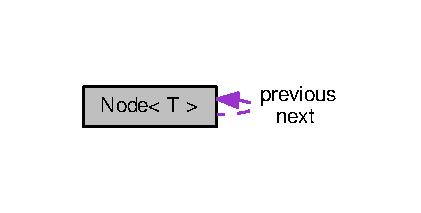
\includegraphics[width=202pt]{classNode__coll__graph}
\end{center}
\end{figure}
\subsection*{Membros públicos}
\begin{DoxyCompactItemize}
\item 
{\bfseries Node} (T data)\hypertarget{classNode_a0692b16d246460bf94c18d49592facdd}{}\label{classNode_a0692b16d246460bf94c18d49592facdd}

\end{DoxyCompactItemize}
\subsection*{Atributos Públicos}
\begin{DoxyCompactItemize}
\item 
T {\bfseries data}\hypertarget{classNode_ac450c71a8677a38d306361f9ced518d3}{}\label{classNode_ac450c71a8677a38d306361f9ced518d3}

\item 
\hyperlink{classNode}{Node} $\ast$ {\bfseries next}\hypertarget{classNode_ac1c0563946c59c36bddde431b4adb00b}{}\label{classNode_ac1c0563946c59c36bddde431b4adb00b}

\item 
\hyperlink{classNode}{Node} $\ast$ {\bfseries previous}\hypertarget{classNode_a36adf1fae9a4a993a348a26c2ba7ad8b}{}\label{classNode_a36adf1fae9a4a993a348a26c2ba7ad8b}

\end{DoxyCompactItemize}


A documentação para esta classe foi gerada a partir do seguinte ficheiro\+:\begin{DoxyCompactItemize}
\item 
include/lista.\+h\end{DoxyCompactItemize}

\hypertarget{classSapo}{}\section{Referência à classe Sapo}
\label{classSapo}\index{Sapo@{Sapo}}


Classe que representa um \hyperlink{classSapo}{Sapo}.  




{\ttfamily \#include $<$sapo.\+h$>$}

\subsection*{Membros públicos}
\begin{DoxyCompactItemize}
\item 
{\bfseries Sapo} (string nome, short int id, int vitorias, int empates, int pulos\+Dados\+Total, int provas\+Disputadas)\hypertarget{classSapo_a07f55b030964376d57c3523035fcbcec}{}\label{classSapo_a07f55b030964376d57c3523035fcbcec}

\item 
{\bfseries Sapo} (int line)\hypertarget{classSapo_ab8cc127ef1e381492aabd0da261fa868}{}\label{classSapo_ab8cc127ef1e381492aabd0da261fa868}

\item 
int {\bfseries pular} ()\hypertarget{classSapo_a59751d925e844fda0719d99939b8be2a}{}\label{classSapo_a59751d925e844fda0719d99939b8be2a}

\item 
void {\bfseries set\+Nome} (string nome)\hypertarget{classSapo_a21384d051b2ddfc06f63405bcafd57b7}{}\label{classSapo_a21384d051b2ddfc06f63405bcafd57b7}

\item 
string {\bfseries get\+Nome} ()\hypertarget{classSapo_acfb11cd24152f00c9a4996f26f3ee39b}{}\label{classSapo_acfb11cd24152f00c9a4996f26f3ee39b}

\item 
void {\bfseries set\+Id} (short int id)\hypertarget{classSapo_a321064f5be7b3df9d421a44a485e9760}{}\label{classSapo_a321064f5be7b3df9d421a44a485e9760}

\item 
int {\bfseries get\+Id} ()\hypertarget{classSapo_aa33722331db1073cbd0faa58445030f9}{}\label{classSapo_aa33722331db1073cbd0faa58445030f9}

\item 
void {\bfseries incrementar\+Vitoria} ()\hypertarget{classSapo_aec1b015f12f87ca82bca5443f527f423}{}\label{classSapo_aec1b015f12f87ca82bca5443f527f423}

\item 
void {\bfseries incrementar\+Provas\+Disputadas} ()\hypertarget{classSapo_a6eabbccc8722c4547d70714d37ad921d}{}\label{classSapo_a6eabbccc8722c4547d70714d37ad921d}

\item 
int {\bfseries get\+Vitorias} ()\hypertarget{classSapo_a102f82c22691765c15873d4ea667156e}{}\label{classSapo_a102f82c22691765c15873d4ea667156e}

\item 
int {\bfseries get\+Empates} ()\hypertarget{classSapo_a24a527ff7ab06d1bde72a76fef41a17c}{}\label{classSapo_a24a527ff7ab06d1bde72a76fef41a17c}

\item 
int {\bfseries get\+Pulos\+Dados\+Total} ()\hypertarget{classSapo_aa8c32cb5b1fbb1516b0a374f63b016a0}{}\label{classSapo_aa8c32cb5b1fbb1516b0a374f63b016a0}

\item 
int {\bfseries get\+Provas\+Disputadas} ()\hypertarget{classSapo_a696fde1a1c0a5dde7f424cb2637d2895}{}\label{classSapo_a696fde1a1c0a5dde7f424cb2637d2895}

\item 
int {\bfseries get\+Distancia\+Percorrida} ()\hypertarget{classSapo_a41a99439aacf25a65c60622eb7e65f60}{}\label{classSapo_a41a99439aacf25a65c60622eb7e65f60}

\item 
int {\bfseries get\+Pulos\+Dados} ()\hypertarget{classSapo_a9b0fa3af63f26b61e822f71afe853e6c}{}\label{classSapo_a9b0fa3af63f26b61e822f71afe853e6c}

\end{DoxyCompactItemize}
\subsection*{Atributos Públicos Estáticos}
\begin{DoxyCompactItemize}
\item 
static std\+::random\+\_\+device {\bfseries rd} \{\}\hypertarget{classSapo_a382c452c69ddad80c4f5b410f1d5687f}{}\label{classSapo_a382c452c69ddad80c4f5b410f1d5687f}

\item 
static std\+::mt19937 {\bfseries gen}\hypertarget{classSapo_ad6855a4e0c711e1a46be2c2609ab0398}{}\label{classSapo_ad6855a4e0c711e1a46be2c2609ab0398}

\item 
static std\+::uniform\+\_\+int\+\_\+distribution {\bfseries dis}\hypertarget{classSapo_a56c768e990e4a2f6ebac183dbc45ce77}{}\label{classSapo_a56c768e990e4a2f6ebac183dbc45ce77}

\item 
static int \hyperlink{classSapo_a27db8e8195d914b42d78114c02fe3fc2}{distancia\+Corrida} = 0
\end{DoxyCompactItemize}
\subsection*{Amigos}
\begin{DoxyCompactItemize}
\item 
istream \& {\bfseries operator$>$$>$} (istream \&i, \hyperlink{classSapo}{Sapo} \&\+\_\+s)\hypertarget{classSapo_a73378689a1d6326dd472e2589f2d0829}{}\label{classSapo_a73378689a1d6326dd472e2589f2d0829}

\item 
ostream \& {\bfseries operator$<$$<$} (ostream \&o, const \hyperlink{classSapo}{Sapo} \&\+\_\+s)\hypertarget{classSapo_aee33b9343a7dc060d778eff236afc8eb}{}\label{classSapo_aee33b9343a7dc060d778eff236afc8eb}

\item 
ofstream \& {\bfseries operator$<$$<$} (ofstream \&of, const \hyperlink{classSapo}{Sapo} \&\+\_\+s)\hypertarget{classSapo_a6d5f849e2bd197bf4b4d10cf4ca428f5}{}\label{classSapo_a6d5f849e2bd197bf4b4d10cf4ca428f5}

\end{DoxyCompactItemize}


\subsection{Descrição detalhada}
Classe que representa um \hyperlink{classSapo}{Sapo}. 

Uma classe com todos os devidos atributos e membros necessários para representar um \hyperlink{classSapo}{Sapo} na corrida. 

\subsection{Documentação dos dados membro}
\index{Sapo@{Sapo}!distancia\+Corrida@{distancia\+Corrida}}
\index{distancia\+Corrida@{distancia\+Corrida}!Sapo@{Sapo}}
\subsubsection[{\texorpdfstring{distancia\+Corrida}{distanciaCorrida}}]{\setlength{\rightskip}{0pt plus 5cm}int Sapo\+::distancia\+Corrida = 0\hspace{0.3cm}{\ttfamily [static]}}\hypertarget{classSapo_a27db8e8195d914b42d78114c02fe3fc2}{}\label{classSapo_a27db8e8195d914b42d78114c02fe3fc2}
static int Variável estática contendo o tamanho da corrida. 

A documentação para esta classe foi gerada a partir dos seguintes ficheiros\+:\begin{DoxyCompactItemize}
\item 
include/\hyperlink{sapo_8h}{sapo.\+h}\item 
src/\hyperlink{main_8cpp}{main.\+cpp}\item 
src/sapo.\+cpp\end{DoxyCompactItemize}

\chapter{Documentação do ficheiro}
\hypertarget{dataManager_8h}{}\section{Referência ao ficheiro include/data\+Manager.h}
\label{dataManager_8h}\index{include/data\+Manager.\+h@{include/data\+Manager.\+h}}


Responsável por carregar e salvar as informaçoes das classes em arquivo.  


{\ttfamily \#include \char`\"{}file\+Handler.\+h\char`\"{}}\\*
{\ttfamily \#include \char`\"{}lista.\+h\char`\"{}}\\*
{\ttfamily \#include \char`\"{}sapo.\+h\char`\"{}}\\*
{\ttfamily \#include \char`\"{}corrida.\+h\char`\"{}}\\*
Diagrama de dependências de inclusão para data\+Manager.\+h\+:\nopagebreak
\begin{figure}[H]
\begin{center}
\leavevmode
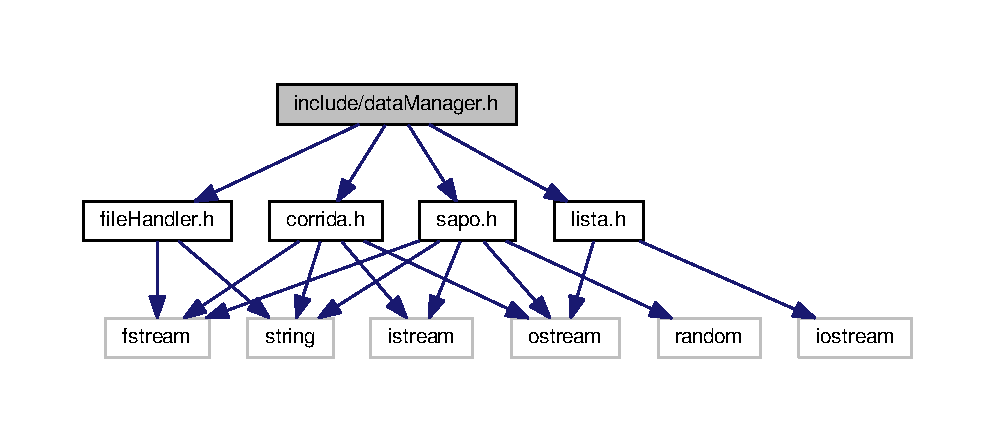
\includegraphics[width=350pt]{dataManager_8h__incl}
\end{center}
\end{figure}
Este grafo mostra quais são os ficheiros que incluem directamente ou indirectamente este ficheiro\+:\nopagebreak
\begin{figure}[H]
\begin{center}
\leavevmode
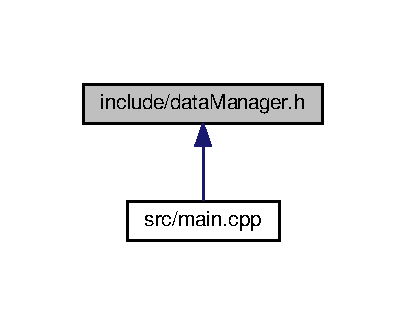
\includegraphics[width=195pt]{dataManager_8h__dep__incl}
\end{center}
\end{figure}
\subsection*{Macros}
\begin{DoxyCompactItemize}
\item 
\#define {\bfseries T\+A\+M\+A\+N\+H\+O\+\_\+\+M\+I\+N\+I\+M\+O\+\_\+\+C\+O\+R\+R\+I\+DA}~100\hypertarget{dataManager_8h_ab19243b566a5c51ae757c231c311fdcb}{}\label{dataManager_8h_ab19243b566a5c51ae757c231c311fdcb}

\item 
\#define {\bfseries T\+A\+M\+A\+N\+H\+O\+\_\+\+M\+A\+X\+I\+M\+O\+\_\+\+C\+O\+R\+R\+I\+DA}~500\hypertarget{dataManager_8h_acd06a70fc4cdc364fdc64990a7cf82c2}{}\label{dataManager_8h_acd06a70fc4cdc364fdc64990a7cf82c2}

\end{DoxyCompactItemize}
\subsection*{Funções}
\begin{DoxyCompactItemize}
\item 
{\footnotesize template$<$typename T $>$ }\\bool \hyperlink{dataManager_8h_a05dd8f0b1643681f147e1f63350a7994}{nome\+Existe} (\hyperlink{classList}{List}$<$ T $>$ $\ast$s, string \&nome, const char $\ast$k)
\begin{DoxyCompactList}\small\item\em Recebe um objeto de Lista, \hyperlink{classSapo}{Sapo} ou \hyperlink{classCorrida}{Corrida}, e verifica se o nome já existe dentro da Lista. \end{DoxyCompactList}\item 
{\footnotesize template$<$typename T $>$ }\\void \hyperlink{dataManager_8h_a1287d4bcfd11e42a9317594b9b67a055}{atualizar\+Dados} (\hyperlink{classList}{List}$<$ T $>$ $\ast$l, const char $\ast$c)
\begin{DoxyCompactList}\small\item\em Azualiza os dados do arquivo. \end{DoxyCompactList}\item 
{\footnotesize template$<$typename T , typename Y $>$ }\\int \hyperlink{dataManager_8h_a18ca9eeda06145dcc9665c0280ea5328}{carregar\+Dados} (\hyperlink{classList}{List}$<$ T $>$ $\ast$l, const char $\ast$c)
\begin{DoxyCompactList}\small\item\em Carrega os dados do arquivo em classes e os insere dentro da Lista. \end{DoxyCompactList}\item 
{\footnotesize template$<$typename T $>$ }\\void \hyperlink{dataManager_8h_a4f92c9c9f7ca2bf8af75dc753854d46a}{salvar\+Dado} (T obj, const char $\ast$c)
\begin{DoxyCompactList}\small\item\em Salva um objeto T no arquivo (onde T pode ser um \hyperlink{classSapo}{Sapo} ou uma \hyperlink{classCorrida}{Corrida}) \end{DoxyCompactList}\item 
void \hyperlink{dataManager_8h_a30f3d19d9141516d7010284a211e211b}{criar\+Sapo} (\hyperlink{classList}{List}$<$ \hyperlink{classSapo}{Sapo} $\ast$ $>$ $\ast$s, int \&id)
\begin{DoxyCompactList}\small\item\em Cria uma classe sapo e a insere na Lista. \end{DoxyCompactList}\item 
void \hyperlink{dataManager_8h_a6967a96d94ca5e70a55419cc4a2609fb}{criar\+Corrida} (\hyperlink{classList}{List}$<$ \hyperlink{classCorrida}{Corrida} $\ast$ $>$ $\ast$c, int \&id)
\begin{DoxyCompactList}\small\item\em Cria uma classe corrida e a insere na Lista. \end{DoxyCompactList}\end{DoxyCompactItemize}


\subsection{Descrição detalhada}
Responsável por carregar e salvar as informaçoes das classes em arquivo. 

\begin{DoxyAuthor}{Autor}
Ariel Oliveira (\href{mailto:ariel.oliveira01@gmail.com}{\tt ariel.\+oliveira01@gmail.\+com}) 
\end{DoxyAuthor}
\begin{DoxySince}{Desde}
20/03/2018 
\end{DoxySince}
\begin{DoxyDate}{Data}
16/06/2018 
\end{DoxyDate}


\subsection{Documentação das funções}
\index{data\+Manager.\+h@{data\+Manager.\+h}!atualizar\+Dados@{atualizar\+Dados}}
\index{atualizar\+Dados@{atualizar\+Dados}!data\+Manager.\+h@{data\+Manager.\+h}}
\subsubsection[{\texorpdfstring{atualizar\+Dados(\+List$<$ T $>$ $\ast$l, const char $\ast$c)}{atualizarDados(List< T > *l, const char *c)}}]{\setlength{\rightskip}{0pt plus 5cm}template$<$typename T $>$ void atualizar\+Dados (
\begin{DoxyParamCaption}
\item[{{\bf List}$<$ T $>$ $\ast$}]{l, }
\item[{const char $\ast$}]{c}
\end{DoxyParamCaption}
)}\hypertarget{dataManager_8h_a1287d4bcfd11e42a9317594b9b67a055}{}\label{dataManager_8h_a1287d4bcfd11e42a9317594b9b67a055}


Azualiza os dados do arquivo. 


\begin{DoxyParams}{Parâmetros}
{\em $\ast$l} & Objeto genérico de uma T\+AD Lista \\
\hline
{\em $\ast$c} & Uma constante de char que contém o diretório do arquivo \\
\hline
\end{DoxyParams}
\begin{DoxyReturn}{Retorna}
void 
\end{DoxyReturn}
\index{data\+Manager.\+h@{data\+Manager.\+h}!carregar\+Dados@{carregar\+Dados}}
\index{carregar\+Dados@{carregar\+Dados}!data\+Manager.\+h@{data\+Manager.\+h}}
\subsubsection[{\texorpdfstring{carregar\+Dados(\+List$<$ T $>$ $\ast$l, const char $\ast$c)}{carregarDados(List< T > *l, const char *c)}}]{\setlength{\rightskip}{0pt plus 5cm}template$<$typename T , typename Y $>$ int carregar\+Dados (
\begin{DoxyParamCaption}
\item[{{\bf List}$<$ T $>$ $\ast$}]{l, }
\item[{const char $\ast$}]{c}
\end{DoxyParamCaption}
)}\hypertarget{dataManager_8h_a18ca9eeda06145dcc9665c0280ea5328}{}\label{dataManager_8h_a18ca9eeda06145dcc9665c0280ea5328}


Carrega os dados do arquivo em classes e os insere dentro da Lista. 


\begin{DoxyParams}{Parâmetros}
{\em $\ast$l} & Objeto genérico de uma T\+AD Lista \\
\hline
{\em $\ast$c} & Uma constante de char que contém o diretório do arquivo \\
\hline
\end{DoxyParams}
\begin{DoxyReturn}{Retorna}
void 
\end{DoxyReturn}
\index{data\+Manager.\+h@{data\+Manager.\+h}!criar\+Corrida@{criar\+Corrida}}
\index{criar\+Corrida@{criar\+Corrida}!data\+Manager.\+h@{data\+Manager.\+h}}
\subsubsection[{\texorpdfstring{criar\+Corrida(\+List$<$ Corrida $\ast$ $>$ $\ast$c, int \&id)}{criarCorrida(List< Corrida * > *c, int &id)}}]{\setlength{\rightskip}{0pt plus 5cm}void criar\+Corrida (
\begin{DoxyParamCaption}
\item[{{\bf List}$<$ {\bf Corrida} $\ast$ $>$ $\ast$}]{c, }
\item[{int \&}]{id}
\end{DoxyParamCaption}
)}\hypertarget{dataManager_8h_a6967a96d94ca5e70a55419cc4a2609fb}{}\label{dataManager_8h_a6967a96d94ca5e70a55419cc4a2609fb}


Cria uma classe corrida e a insere na Lista. 


\begin{DoxyParams}{Parâmetros}
{\em $\ast$s} & Objeto de uma classe (\hyperlink{classCorrida}{Corrida}) \\
\hline
{\em \&id} & Inteiro que representa o ID da próximo corrida a ser inserida na lista \\
\hline
\end{DoxyParams}
\begin{DoxyReturn}{Retorna}
void 
\end{DoxyReturn}
\index{data\+Manager.\+h@{data\+Manager.\+h}!criar\+Sapo@{criar\+Sapo}}
\index{criar\+Sapo@{criar\+Sapo}!data\+Manager.\+h@{data\+Manager.\+h}}
\subsubsection[{\texorpdfstring{criar\+Sapo(\+List$<$ Sapo $\ast$ $>$ $\ast$s, int \&id)}{criarSapo(List< Sapo * > *s, int &id)}}]{\setlength{\rightskip}{0pt plus 5cm}void criar\+Sapo (
\begin{DoxyParamCaption}
\item[{{\bf List}$<$ {\bf Sapo} $\ast$ $>$ $\ast$}]{s, }
\item[{int \&}]{id}
\end{DoxyParamCaption}
)}\hypertarget{dataManager_8h_a30f3d19d9141516d7010284a211e211b}{}\label{dataManager_8h_a30f3d19d9141516d7010284a211e211b}


Cria uma classe sapo e a insere na Lista. 


\begin{DoxyParams}{Parâmetros}
{\em $\ast$s} & Objeto de uma classe (\hyperlink{classSapo}{Sapo}) \\
\hline
{\em \&id} & Inteiro que representa o ID do próximo sapo a ser inserido na lista \\
\hline
\end{DoxyParams}
\begin{DoxyReturn}{Retorna}
void 
\end{DoxyReturn}
\index{data\+Manager.\+h@{data\+Manager.\+h}!nome\+Existe@{nome\+Existe}}
\index{nome\+Existe@{nome\+Existe}!data\+Manager.\+h@{data\+Manager.\+h}}
\subsubsection[{\texorpdfstring{nome\+Existe(\+List$<$ T $>$ $\ast$s, string \&nome, const char $\ast$k)}{nomeExiste(List< T > *s, string &nome, const char *k)}}]{\setlength{\rightskip}{0pt plus 5cm}template$<$typename T $>$ bool nome\+Existe (
\begin{DoxyParamCaption}
\item[{{\bf List}$<$ T $>$ $\ast$}]{s, }
\item[{string \&}]{nome, }
\item[{const char $\ast$}]{k}
\end{DoxyParamCaption}
)}\hypertarget{dataManager_8h_a05dd8f0b1643681f147e1f63350a7994}{}\label{dataManager_8h_a05dd8f0b1643681f147e1f63350a7994}


Recebe um objeto de Lista, \hyperlink{classSapo}{Sapo} ou \hyperlink{classCorrida}{Corrida}, e verifica se o nome já existe dentro da Lista. 


\begin{DoxyParams}{Parâmetros}
{\em $\ast$s} & Objeto genérico de uma T\+AD Lista \\
\hline
{\em \&nome} & Uma string contendo o nome a ser comparado \\
\hline
{\em $\ast$k} & Uma constante de char que será impresso na tela \\
\hline
\end{DoxyParams}
\begin{DoxyReturn}{Retorna}
true Se o nome existir. Caso contrário, retorna false. 
\end{DoxyReturn}
\index{data\+Manager.\+h@{data\+Manager.\+h}!salvar\+Dado@{salvar\+Dado}}
\index{salvar\+Dado@{salvar\+Dado}!data\+Manager.\+h@{data\+Manager.\+h}}
\subsubsection[{\texorpdfstring{salvar\+Dado(\+T obj, const char $\ast$c)}{salvarDado(T obj, const char *c)}}]{\setlength{\rightskip}{0pt plus 5cm}template$<$typename T $>$ void salvar\+Dado (
\begin{DoxyParamCaption}
\item[{T}]{obj, }
\item[{const char $\ast$}]{c}
\end{DoxyParamCaption}
)}\hypertarget{dataManager_8h_a4f92c9c9f7ca2bf8af75dc753854d46a}{}\label{dataManager_8h_a4f92c9c9f7ca2bf8af75dc753854d46a}


Salva um objeto T no arquivo (onde T pode ser um \hyperlink{classSapo}{Sapo} ou uma \hyperlink{classCorrida}{Corrida}) 


\begin{DoxyParams}{Parâmetros}
{\em obj} & Objeto de uma classe (\hyperlink{classSapo}{Sapo} ou \hyperlink{classCorrida}{Corrida}) \\
\hline
{\em $\ast$c} & Uma constante de char que contém o diretório do arquivo \\
\hline
\end{DoxyParams}
\begin{DoxyReturn}{Retorna}
void 
\end{DoxyReturn}

\hypertarget{fileHandler_8h}{}\section{Referência ao ficheiro include/file\+Handler.h}
\label{fileHandler_8h}\index{include/file\+Handler.\+h@{include/file\+Handler.\+h}}


Responsável por manipular os arquivos C\+SV.  


{\ttfamily \#include $<$fstream$>$}\\*
{\ttfamily \#include $<$string$>$}\\*
Diagrama de dependências de inclusão para file\+Handler.\+h\+:\nopagebreak
\begin{figure}[H]
\begin{center}
\leavevmode
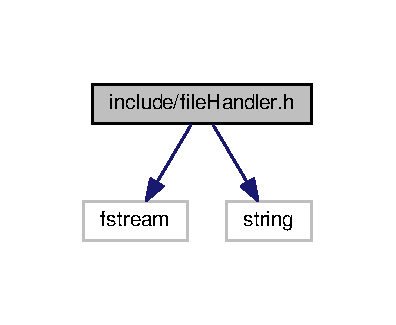
\includegraphics[width=190pt]{fileHandler_8h__incl}
\end{center}
\end{figure}
Este grafo mostra quais são os ficheiros que incluem directamente ou indirectamente este ficheiro\+:\nopagebreak
\begin{figure}[H]
\begin{center}
\leavevmode
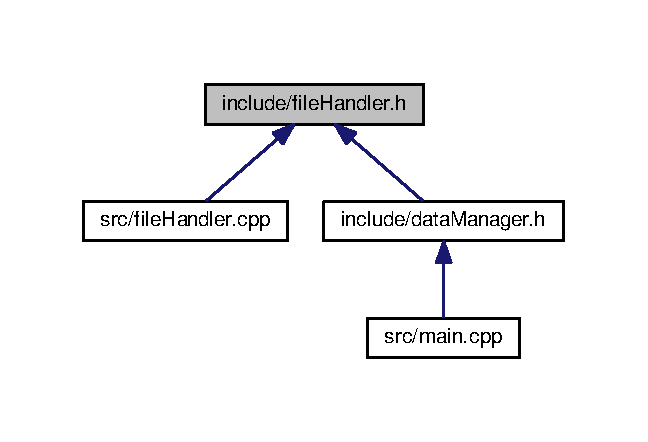
\includegraphics[width=311pt]{fileHandler_8h__dep__incl}
\end{center}
\end{figure}
\subsection*{Funções}
\begin{DoxyCompactItemize}
\item 
void \hyperlink{fileHandler_8h_a998b13a84c814fcf4d7929f9d3811856}{read\+C\+S\+V\+File} (ifstream \&file, int line)
\begin{DoxyCompactList}\small\item\em Acessa a linha do arquivo especificada no parametro line. \end{DoxyCompactList}\item 
void \hyperlink{fileHandler_8h_a66afd072156bee0cffe94e300306f273}{reset\+Stream\+Cursor} (ifstream \&file)
\begin{DoxyCompactList}\small\item\em Coloca o cursor do stream no início do arquivo. \end{DoxyCompactList}\end{DoxyCompactItemize}


\subsection{Descrição detalhada}
Responsável por manipular os arquivos C\+SV. 

\begin{DoxyAuthor}{Autor}
Ariel Oliveira (\href{mailto:ariel.oliveira01@gmail.com}{\tt ariel.\+oliveira01@gmail.\+com}) 
\end{DoxyAuthor}
\begin{DoxySince}{Desde}
20/03/2018 
\end{DoxySince}
\begin{DoxyDate}{Data}
16/06/2018 
\end{DoxyDate}


\subsection{Documentação das funções}
\index{file\+Handler.\+h@{file\+Handler.\+h}!read\+C\+S\+V\+File@{read\+C\+S\+V\+File}}
\index{read\+C\+S\+V\+File@{read\+C\+S\+V\+File}!file\+Handler.\+h@{file\+Handler.\+h}}
\subsubsection[{\texorpdfstring{read\+C\+S\+V\+File(ifstream \&file, int line)}{readCSVFile(ifstream &file, int line)}}]{\setlength{\rightskip}{0pt plus 5cm}void read\+C\+S\+V\+File (
\begin{DoxyParamCaption}
\item[{ifstream \&}]{file, }
\item[{int}]{line}
\end{DoxyParamCaption}
)}\hypertarget{fileHandler_8h_a998b13a84c814fcf4d7929f9d3811856}{}\label{fileHandler_8h_a998b13a84c814fcf4d7929f9d3811856}


Acessa a linha do arquivo especificada no parametro line. 


\begin{DoxyParams}{Parâmetros}
{\em \&file} & Contém o stream do arquivo \\
\hline
{\em $\ast$l} & Inteiro que representa a linha a ser acessada \\
\hline
\end{DoxyParams}
\begin{DoxyReturn}{Retorna}
void 
\end{DoxyReturn}
\index{file\+Handler.\+h@{file\+Handler.\+h}!reset\+Stream\+Cursor@{reset\+Stream\+Cursor}}
\index{reset\+Stream\+Cursor@{reset\+Stream\+Cursor}!file\+Handler.\+h@{file\+Handler.\+h}}
\subsubsection[{\texorpdfstring{reset\+Stream\+Cursor(ifstream \&file)}{resetStreamCursor(ifstream &file)}}]{\setlength{\rightskip}{0pt plus 5cm}void reset\+Stream\+Cursor (
\begin{DoxyParamCaption}
\item[{ifstream \&}]{file}
\end{DoxyParamCaption}
)}\hypertarget{fileHandler_8h_a66afd072156bee0cffe94e300306f273}{}\label{fileHandler_8h_a66afd072156bee0cffe94e300306f273}


Coloca o cursor do stream no início do arquivo. 


\begin{DoxyParams}{Parâmetros}
{\em \&file} & Contém o stream do arquivo \\
\hline
\end{DoxyParams}
\begin{DoxyReturn}{Retorna}
void 
\end{DoxyReturn}

\hypertarget{sapo_8h}{}\section{Referência ao ficheiro include/sapo.h}
\label{sapo_8h}\index{include/sapo.\+h@{include/sapo.\+h}}


Cabeçalho contendo a definição da classe sapo.  


{\ttfamily \#include $<$random$>$}\\*
{\ttfamily \#include $<$string$>$}\\*
{\ttfamily \#include $<$fstream$>$}\\*
{\ttfamily \#include $<$istream$>$}\\*
{\ttfamily \#include $<$ostream$>$}\\*
Diagrama de dependências de inclusão para sapo.\+h\+:\nopagebreak
\begin{figure}[H]
\begin{center}
\leavevmode
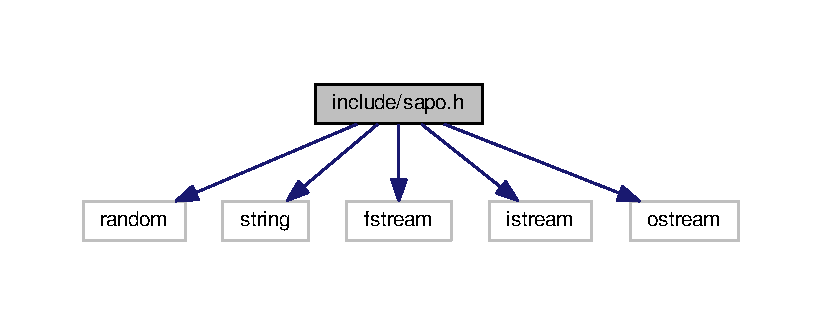
\includegraphics[width=350pt]{sapo_8h__incl}
\end{center}
\end{figure}
Este grafo mostra quais são os ficheiros que incluem directamente ou indirectamente este ficheiro\+:\nopagebreak
\begin{figure}[H]
\begin{center}
\leavevmode
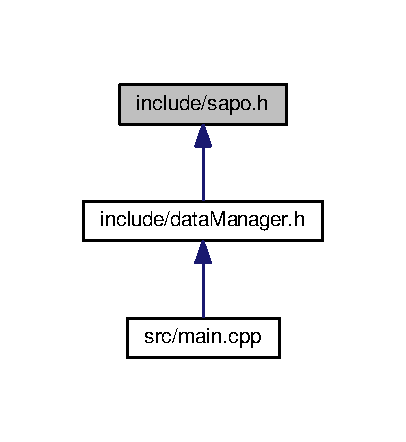
\includegraphics[width=195pt]{sapo_8h__dep__incl}
\end{center}
\end{figure}
\subsection*{Componentes}
\begin{DoxyCompactItemize}
\item 
class \hyperlink{classSapo}{Sapo}
\begin{DoxyCompactList}\small\item\em Classe que representa um \hyperlink{classSapo}{Sapo}. \end{DoxyCompactList}\end{DoxyCompactItemize}


\subsection{Descrição detalhada}
Cabeçalho contendo a definição da classe sapo. 

\begin{DoxyAuthor}{Autor}
Ariel Oliveira (\href{mailto:ariel.oliveira01@gmail.com}{\tt ariel.\+oliveira01@gmail.\+com}) 
\end{DoxyAuthor}
\begin{DoxySince}{Desde}
20/03/2018 
\end{DoxySince}
\begin{DoxyDate}{Data}
16/06/2018 
\end{DoxyDate}

\hypertarget{fileHandler_8cpp}{}\section{Referência ao ficheiro src/file\+Handler.cpp}
\label{fileHandler_8cpp}\index{src/file\+Handler.\+cpp@{src/file\+Handler.\+cpp}}


Responsável por manipular os arquivos C\+SV.  


{\ttfamily \#include \char`\"{}file\+Handler.\+h\char`\"{}}\\*
Diagrama de dependências de inclusão para file\+Handler.\+cpp\+:\nopagebreak
\begin{figure}[H]
\begin{center}
\leavevmode
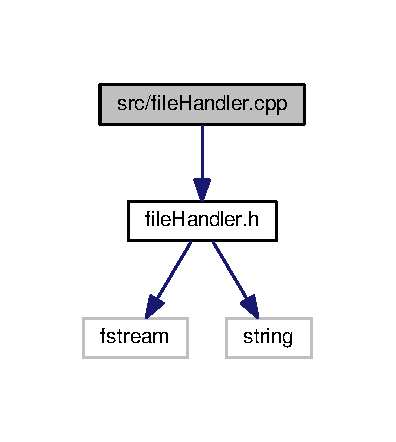
\includegraphics[width=190pt]{fileHandler_8cpp__incl}
\end{center}
\end{figure}
\subsection*{Funções}
\begin{DoxyCompactItemize}
\item 
void \hyperlink{fileHandler_8cpp_a998b13a84c814fcf4d7929f9d3811856}{read\+C\+S\+V\+File} (ifstream \&file, int line)
\begin{DoxyCompactList}\small\item\em Acessa a linha do arquivo especificada no parametro line. \end{DoxyCompactList}\item 
void \hyperlink{fileHandler_8cpp_a66afd072156bee0cffe94e300306f273}{reset\+Stream\+Cursor} (ifstream \&file)
\begin{DoxyCompactList}\small\item\em Coloca o cursor do stream no início do arquivo. \end{DoxyCompactList}\end{DoxyCompactItemize}


\subsection{Descrição detalhada}
Responsável por manipular os arquivos C\+SV. 

Contém a implementaçao das funçoes. \begin{DoxyAuthor}{Autor}
Ariel Oliveira (\href{mailto:ariel.oliveira01@gmail.com}{\tt ariel.\+oliveira01@gmail.\+com}) 
\end{DoxyAuthor}
\begin{DoxySince}{Desde}
20/03/2018 
\end{DoxySince}
\begin{DoxyDate}{Data}
16/06/2018 
\end{DoxyDate}


\subsection{Documentação das funções}
\index{file\+Handler.\+cpp@{file\+Handler.\+cpp}!read\+C\+S\+V\+File@{read\+C\+S\+V\+File}}
\index{read\+C\+S\+V\+File@{read\+C\+S\+V\+File}!file\+Handler.\+cpp@{file\+Handler.\+cpp}}
\subsubsection[{\texorpdfstring{read\+C\+S\+V\+File(ifstream \&file, int line)}{readCSVFile(ifstream &file, int line)}}]{\setlength{\rightskip}{0pt plus 5cm}void read\+C\+S\+V\+File (
\begin{DoxyParamCaption}
\item[{ifstream \&}]{file, }
\item[{int}]{line}
\end{DoxyParamCaption}
)}\hypertarget{fileHandler_8cpp_a998b13a84c814fcf4d7929f9d3811856}{}\label{fileHandler_8cpp_a998b13a84c814fcf4d7929f9d3811856}


Acessa a linha do arquivo especificada no parametro line. 


\begin{DoxyParams}{Parâmetros}
{\em \&file} & Contém o stream do arquivo \\
\hline
{\em $\ast$l} & Inteiro que representa a linha a ser acessada \\
\hline
\end{DoxyParams}
\begin{DoxyReturn}{Retorna}
void 
\end{DoxyReturn}
\index{file\+Handler.\+cpp@{file\+Handler.\+cpp}!reset\+Stream\+Cursor@{reset\+Stream\+Cursor}}
\index{reset\+Stream\+Cursor@{reset\+Stream\+Cursor}!file\+Handler.\+cpp@{file\+Handler.\+cpp}}
\subsubsection[{\texorpdfstring{reset\+Stream\+Cursor(ifstream \&file)}{resetStreamCursor(ifstream &file)}}]{\setlength{\rightskip}{0pt plus 5cm}void reset\+Stream\+Cursor (
\begin{DoxyParamCaption}
\item[{ifstream \&}]{file}
\end{DoxyParamCaption}
)}\hypertarget{fileHandler_8cpp_a66afd072156bee0cffe94e300306f273}{}\label{fileHandler_8cpp_a66afd072156bee0cffe94e300306f273}


Coloca o cursor do stream no início do arquivo. 


\begin{DoxyParams}{Parâmetros}
{\em \&file} & Contém o stream do arquivo \\
\hline
\end{DoxyParams}
\begin{DoxyReturn}{Retorna}
void 
\end{DoxyReturn}

\hypertarget{main_8cpp}{}\section{Referência ao ficheiro src/main.cpp}
\label{main_8cpp}\index{src/main.\+cpp@{src/main.\+cpp}}


Programa que simula uma corrida de sapos.  


{\ttfamily \#include $<$iostream$>$}\\*
{\ttfamily \#include $<$sstream$>$}\\*
{\ttfamily \#include \char`\"{}data\+Manager.\+h\char`\"{}}\\*
Diagrama de dependências de inclusão para main.\+cpp\+:\nopagebreak
\begin{figure}[H]
\begin{center}
\leavevmode
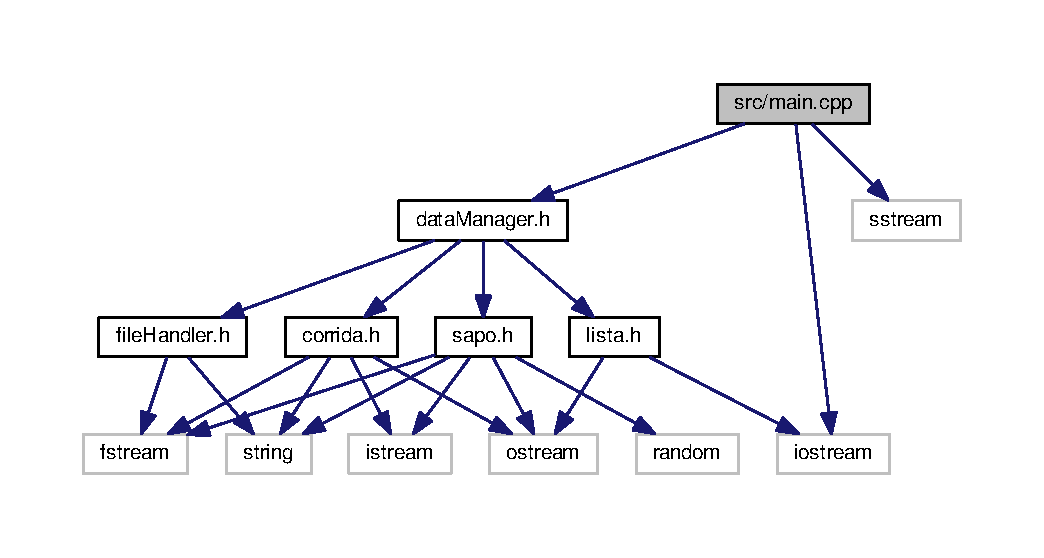
\includegraphics[width=350pt]{main_8cpp__incl}
\end{center}
\end{figure}
\subsection*{Enumerações}
\begin{DoxyCompactItemize}
\item 
enum \hyperlink{main_8cpp_af3d52afbb0d088f62e02208b24a9cbd2}{Menu} \{ \\*
{\bfseries N\+U\+LO}, 
{\bfseries S\+A\+P\+O\+\_\+\+S\+T\+A\+TS}, 
{\bfseries C\+O\+R\+R\+I\+D\+A\+\_\+\+S\+T\+A\+TS}, 
{\bfseries I\+N\+I\+C\+I\+AR}, 
\\*
{\bfseries C\+R\+I\+A\+R\+\_\+\+S\+A\+PO}, 
{\bfseries C\+R\+I\+A\+R\+\_\+\+C\+O\+R\+R\+I\+DA}, 
{\bfseries S\+A\+IR}
 \}
\end{DoxyCompactItemize}
\subsection*{Funções}
\begin{DoxyCompactItemize}
\item 
bool \hyperlink{main_8cpp_ac9da77b344fdfbf80e44ac41e5eee7b1}{venceu} (\hyperlink{classSapo}{Sapo} $\ast$sapo)
\begin{DoxyCompactList}\small\item\em Verifica se o sapo passou a linha de chegada. \end{DoxyCompactList}\item 
bool \hyperlink{main_8cpp_a453c6d4383f08d8b257d58404342d5a4}{empatou} (\hyperlink{classSapo}{Sapo} $\ast$s1, \hyperlink{classSapo}{Sapo} $\ast$s2)
\begin{DoxyCompactList}\small\item\em Verifica se o sapo s1 e s2 estão em condição de empate. \end{DoxyCompactList}\item 
void \hyperlink{main_8cpp_a215a710d0178dcac06cfd5f1ebaa272e}{mostrar\+Ranking} (\hyperlink{classList}{List}$<$ \hyperlink{classSapo}{Sapo} $\ast$ $>$ $\ast$finalistas)
\begin{DoxyCompactList}\small\item\em Mostra o ranking dos sapos na ordem de chegada. \end{DoxyCompactList}\item 
void \hyperlink{main_8cpp_a0de112b9364672d94de3e2475e8a7480}{exibir\+Sapos\+Stats} (\hyperlink{classList}{List}$<$ \hyperlink{classSapo}{Sapo} $\ast$ $>$ $\ast$s)
\begin{DoxyCompactList}\small\item\em Mostra a lista de sapos carregados no programa. \end{DoxyCompactList}\item 
void \hyperlink{main_8cpp_af69f7dd90750aa96d2ce8d503a6a6a7c}{exibir\+Corridas\+Stats} (\hyperlink{classList}{List}$<$ \hyperlink{classCorrida}{Corrida} $\ast$ $>$ $\ast$c)
\begin{DoxyCompactList}\small\item\em Mostra a lista de corridas carregadas no programa. \end{DoxyCompactList}\item 
void \hyperlink{main_8cpp_a7e9505121fc1732c838abc02e34dfd23}{determinar\+Vencedor} (\hyperlink{classList}{List}$<$ \hyperlink{classSapo}{Sapo} $\ast$ $>$ $\ast$s)
\begin{DoxyCompactList}\small\item\em Executa a corrida propriamente dita, determinando o sapo vencedor. \end{DoxyCompactList}\item 
int \hyperlink{main_8cpp_a2510281af08509eb98249bbe7d75af91}{escolher\+Corrida} (\hyperlink{classList}{List}$<$ \hyperlink{classCorrida}{Corrida} $\ast$ $>$ $\ast$c)
\begin{DoxyCompactList}\small\item\em Mostra um menu de escolha das corridas para o usuário. \end{DoxyCompactList}\item 
void \hyperlink{main_8cpp_a2a0e843767aeea4f433a28b9c54f573a}{menu} ()
\begin{DoxyCompactList}\small\item\em Exibe o menu principal do programa. \end{DoxyCompactList}\item 
int {\bfseries main} ()\hypertarget{main_8cpp_ae66f6b31b5ad750f1fe042a706a4e3d4}{}\label{main_8cpp_ae66f6b31b5ad750f1fe042a706a4e3d4}

\end{DoxyCompactItemize}


\subsection{Descrição detalhada}
Programa que simula uma corrida de sapos. 

\begin{DoxyAuthor}{Autor}
Ariel Oliveira (\href{mailto:ariel.oliveira01@gmail.com}{\tt ariel.\+oliveira01@gmail.\+com}) 
\end{DoxyAuthor}
\begin{DoxySince}{Desde}
20/03/2018 
\end{DoxySince}
\begin{DoxyDate}{Data}
16/06/2018 
\end{DoxyDate}


\subsection{Documentação dos valores da enumeração}
\index{main.\+cpp@{main.\+cpp}!Menu@{Menu}}
\index{Menu@{Menu}!main.\+cpp@{main.\+cpp}}
\subsubsection[{\texorpdfstring{Menu}{Menu}}]{\setlength{\rightskip}{0pt plus 5cm}enum {\bf Menu}}\hypertarget{main_8cpp_af3d52afbb0d088f62e02208b24a9cbd2}{}\label{main_8cpp_af3d52afbb0d088f62e02208b24a9cbd2}
Enum Menu Uma enumeração com as opções do menu principal. 

\subsection{Documentação das funções}
\index{main.\+cpp@{main.\+cpp}!determinar\+Vencedor@{determinar\+Vencedor}}
\index{determinar\+Vencedor@{determinar\+Vencedor}!main.\+cpp@{main.\+cpp}}
\subsubsection[{\texorpdfstring{determinar\+Vencedor(\+List$<$ Sapo $\ast$ $>$ $\ast$s)}{determinarVencedor(List< Sapo * > *s)}}]{\setlength{\rightskip}{0pt plus 5cm}void determinar\+Vencedor (
\begin{DoxyParamCaption}
\item[{{\bf List}$<$ {\bf Sapo} $\ast$ $>$ $\ast$}]{s}
\end{DoxyParamCaption}
)}\hypertarget{main_8cpp_a7e9505121fc1732c838abc02e34dfd23}{}\label{main_8cpp_a7e9505121fc1732c838abc02e34dfd23}


Executa a corrida propriamente dita, determinando o sapo vencedor. 


\begin{DoxyParams}{Parâmetros}
{\em $\ast$s} & Objeto de uma T\+AD \hyperlink{classList}{List} contendo os sapos a competir \\
\hline
\end{DoxyParams}
\begin{DoxyReturn}{Retorna}
void 
\end{DoxyReturn}
\index{main.\+cpp@{main.\+cpp}!empatou@{empatou}}
\index{empatou@{empatou}!main.\+cpp@{main.\+cpp}}
\subsubsection[{\texorpdfstring{empatou(\+Sapo $\ast$s1, Sapo $\ast$s2)}{empatou(Sapo *s1, Sapo *s2)}}]{\setlength{\rightskip}{0pt plus 5cm}bool empatou (
\begin{DoxyParamCaption}
\item[{{\bf Sapo} $\ast$}]{s1, }
\item[{{\bf Sapo} $\ast$}]{s2}
\end{DoxyParamCaption}
)}\hypertarget{main_8cpp_a453c6d4383f08d8b257d58404342d5a4}{}\label{main_8cpp_a453c6d4383f08d8b257d58404342d5a4}


Verifica se o sapo s1 e s2 estão em condição de empate. 


\begin{DoxyParams}{Parâmetros}
{\em $\ast$s1} & Objeto da classe \hyperlink{classSapo}{Sapo} \\
\hline
{\em $\ast$s2} & Objeto da classe \hyperlink{classSapo}{Sapo} \\
\hline
\end{DoxyParams}
\begin{DoxyReturn}{Retorna}
true Se os sapos estiverem na condição tratada 
\end{DoxyReturn}
\index{main.\+cpp@{main.\+cpp}!escolher\+Corrida@{escolher\+Corrida}}
\index{escolher\+Corrida@{escolher\+Corrida}!main.\+cpp@{main.\+cpp}}
\subsubsection[{\texorpdfstring{escolher\+Corrida(\+List$<$ Corrida $\ast$ $>$ $\ast$c)}{escolherCorrida(List< Corrida * > *c)}}]{\setlength{\rightskip}{0pt plus 5cm}int escolher\+Corrida (
\begin{DoxyParamCaption}
\item[{{\bf List}$<$ {\bf Corrida} $\ast$ $>$ $\ast$}]{c}
\end{DoxyParamCaption}
)}\hypertarget{main_8cpp_a2510281af08509eb98249bbe7d75af91}{}\label{main_8cpp_a2510281af08509eb98249bbe7d75af91}


Mostra um menu de escolha das corridas para o usuário. 


\begin{DoxyParams}{Parâmetros}
{\em $\ast$} & Objeto de uma T\+AD \hyperlink{classList}{List} contendo as corridas \\
\hline
\end{DoxyParams}
\begin{DoxyReturn}{Retorna}
int Opção escolhida pelo usuário 
\end{DoxyReturn}
\index{main.\+cpp@{main.\+cpp}!exibir\+Corridas\+Stats@{exibir\+Corridas\+Stats}}
\index{exibir\+Corridas\+Stats@{exibir\+Corridas\+Stats}!main.\+cpp@{main.\+cpp}}
\subsubsection[{\texorpdfstring{exibir\+Corridas\+Stats(\+List$<$ Corrida $\ast$ $>$ $\ast$c)}{exibirCorridasStats(List< Corrida * > *c)}}]{\setlength{\rightskip}{0pt plus 5cm}void exibir\+Corridas\+Stats (
\begin{DoxyParamCaption}
\item[{{\bf List}$<$ {\bf Corrida} $\ast$ $>$ $\ast$}]{c}
\end{DoxyParamCaption}
)}\hypertarget{main_8cpp_af69f7dd90750aa96d2ce8d503a6a6a7c}{}\label{main_8cpp_af69f7dd90750aa96d2ce8d503a6a6a7c}


Mostra a lista de corridas carregadas no programa. 


\begin{DoxyParams}{Parâmetros}
{\em $\ast$c} & Objeto de uma T\+AD \hyperlink{classList}{List} \\
\hline
\end{DoxyParams}
\begin{DoxyReturn}{Retorna}
void 
\end{DoxyReturn}
\index{main.\+cpp@{main.\+cpp}!exibir\+Sapos\+Stats@{exibir\+Sapos\+Stats}}
\index{exibir\+Sapos\+Stats@{exibir\+Sapos\+Stats}!main.\+cpp@{main.\+cpp}}
\subsubsection[{\texorpdfstring{exibir\+Sapos\+Stats(\+List$<$ Sapo $\ast$ $>$ $\ast$s)}{exibirSaposStats(List< Sapo * > *s)}}]{\setlength{\rightskip}{0pt plus 5cm}void exibir\+Sapos\+Stats (
\begin{DoxyParamCaption}
\item[{{\bf List}$<$ {\bf Sapo} $\ast$ $>$ $\ast$}]{s}
\end{DoxyParamCaption}
)}\hypertarget{main_8cpp_a0de112b9364672d94de3e2475e8a7480}{}\label{main_8cpp_a0de112b9364672d94de3e2475e8a7480}


Mostra a lista de sapos carregados no programa. 


\begin{DoxyParams}{Parâmetros}
{\em $\ast$s} & Objeto de uma T\+AD \hyperlink{classList}{List} \\
\hline
\end{DoxyParams}
\begin{DoxyReturn}{Retorna}
void 
\end{DoxyReturn}
\index{main.\+cpp@{main.\+cpp}!menu@{menu}}
\index{menu@{menu}!main.\+cpp@{main.\+cpp}}
\subsubsection[{\texorpdfstring{menu()}{menu()}}]{\setlength{\rightskip}{0pt plus 5cm}void menu (
\begin{DoxyParamCaption}
{}
\end{DoxyParamCaption}
)}\hypertarget{main_8cpp_a2a0e843767aeea4f433a28b9c54f573a}{}\label{main_8cpp_a2a0e843767aeea4f433a28b9c54f573a}


Exibe o menu principal do programa. 

\begin{DoxyReturn}{Retorna}
int Opção escolhida pelo usuário 
\end{DoxyReturn}
\index{main.\+cpp@{main.\+cpp}!mostrar\+Ranking@{mostrar\+Ranking}}
\index{mostrar\+Ranking@{mostrar\+Ranking}!main.\+cpp@{main.\+cpp}}
\subsubsection[{\texorpdfstring{mostrar\+Ranking(\+List$<$ Sapo $\ast$ $>$ $\ast$finalistas)}{mostrarRanking(List< Sapo * > *finalistas)}}]{\setlength{\rightskip}{0pt plus 5cm}void mostrar\+Ranking (
\begin{DoxyParamCaption}
\item[{{\bf List}$<$ {\bf Sapo} $\ast$ $>$ $\ast$}]{finalistas}
\end{DoxyParamCaption}
)}\hypertarget{main_8cpp_a215a710d0178dcac06cfd5f1ebaa272e}{}\label{main_8cpp_a215a710d0178dcac06cfd5f1ebaa272e}


Mostra o ranking dos sapos na ordem de chegada. 


\begin{DoxyParams}{Parâmetros}
{\em $\ast$finalistas} & Objeto de uma T\+AD \hyperlink{classList}{List} \\
\hline
\end{DoxyParams}
\begin{DoxyReturn}{Retorna}
void 
\end{DoxyReturn}
\index{main.\+cpp@{main.\+cpp}!venceu@{venceu}}
\index{venceu@{venceu}!main.\+cpp@{main.\+cpp}}
\subsubsection[{\texorpdfstring{venceu(\+Sapo $\ast$sapo)}{venceu(Sapo *sapo)}}]{\setlength{\rightskip}{0pt plus 5cm}bool venceu (
\begin{DoxyParamCaption}
\item[{{\bf Sapo} $\ast$}]{sapo}
\end{DoxyParamCaption}
)}\hypertarget{main_8cpp_ac9da77b344fdfbf80e44ac41e5eee7b1}{}\label{main_8cpp_ac9da77b344fdfbf80e44ac41e5eee7b1}


Verifica se o sapo passou a linha de chegada. 


\begin{DoxyParams}{Parâmetros}
{\em $\ast$sapo} & Objeto da classe \hyperlink{classSapo}{Sapo} \\
\hline
\end{DoxyParams}
\begin{DoxyReturn}{Retorna}
true Caso o sapo tenha ganhado 
\end{DoxyReturn}

%--- End generated contents ---

% Index
\backmatter
\newpage
\phantomsection
\clearemptydoublepage
\addcontentsline{toc}{chapter}{Índice}
\printindex

\end{document}
